\section{Recurrent Neural Networks}

\subsection{RNN: Process Sequences}

\paragraph{Overview}

所谓循环神经网络，可以看作是有时序性的神经网络，有时序电路的那种感觉。

\begin{figure}[H]
    \centering
    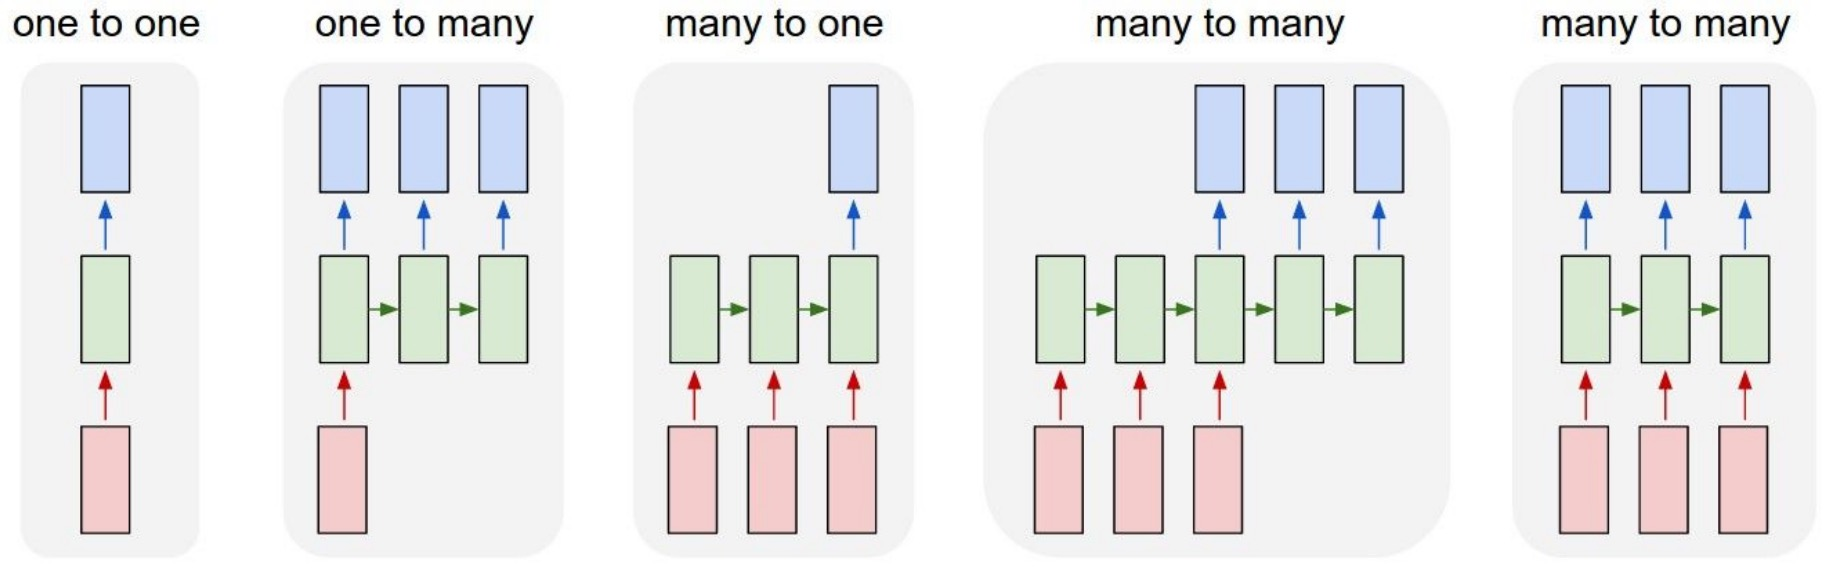
\includegraphics[width=0.8\linewidth]{figs/chapter5/RNN.jpg}
\end{figure}

上图中，横向从左到右可以看作为若干时刻。普通的神经网络是 one to one 的结构——一个输入层，经过一系列隐藏层，到达一个输出层，这些步骤都是在一个时刻完成的；而 RNN 可以处理序列型的数据，其可以是 one to many, many to one, many to many 等结构。

\begin{itemize}[leftmargin=*]
    \item one to many: 某一时刻给一个输入，在之后的若干时刻都有输出。例如 image captioning.
    \item many to one: 在连续的几个时刻给输入，直到最后一个时刻给出输出。例如 audio prediction.
    \item many to many: 在连续的几个时刻给输入，在之后的若干时刻都有输出。例如 video captioning.
    \item many to many: 在连续的几个时刻给输入，同时不断地输出。例如 frame level video classification.
\end{itemize}

\paragraph{Forward}

RNN 向前传播的 key idea 是：每一个神经元有一个“隐藏”的和时序相关的向量 $h_t$，它根据某\textbf{不随时序变化}的参数 $W$ 和当前的输入 $x_t$ 更新，即：
\[
h_t=f_W(h_{t-1}, x_t)
\]
随后可以根据情况（one to many / many to one / many to many）决定如何用 $h_t$ 去更新输出 $y_t$.

例如，一个简单的情形可以是：
\begin{align*}
h_t&=\tanh(W_{hh}h_{t-1}+W_{xh}x_t)\\
y_t&=W_{hy}h_t
\end{align*}

\paragraph{Computational Graph}

为了方便 Backpropagation 的推导，computational graph 是非常重要的技巧。显然，对于不同结构（one to many / many to one / many to many, etc.），它们的 computational graph 会不同，但大同小异：

\begin{figure}[H]
    \centering
    \begin{tabular}{cc}
        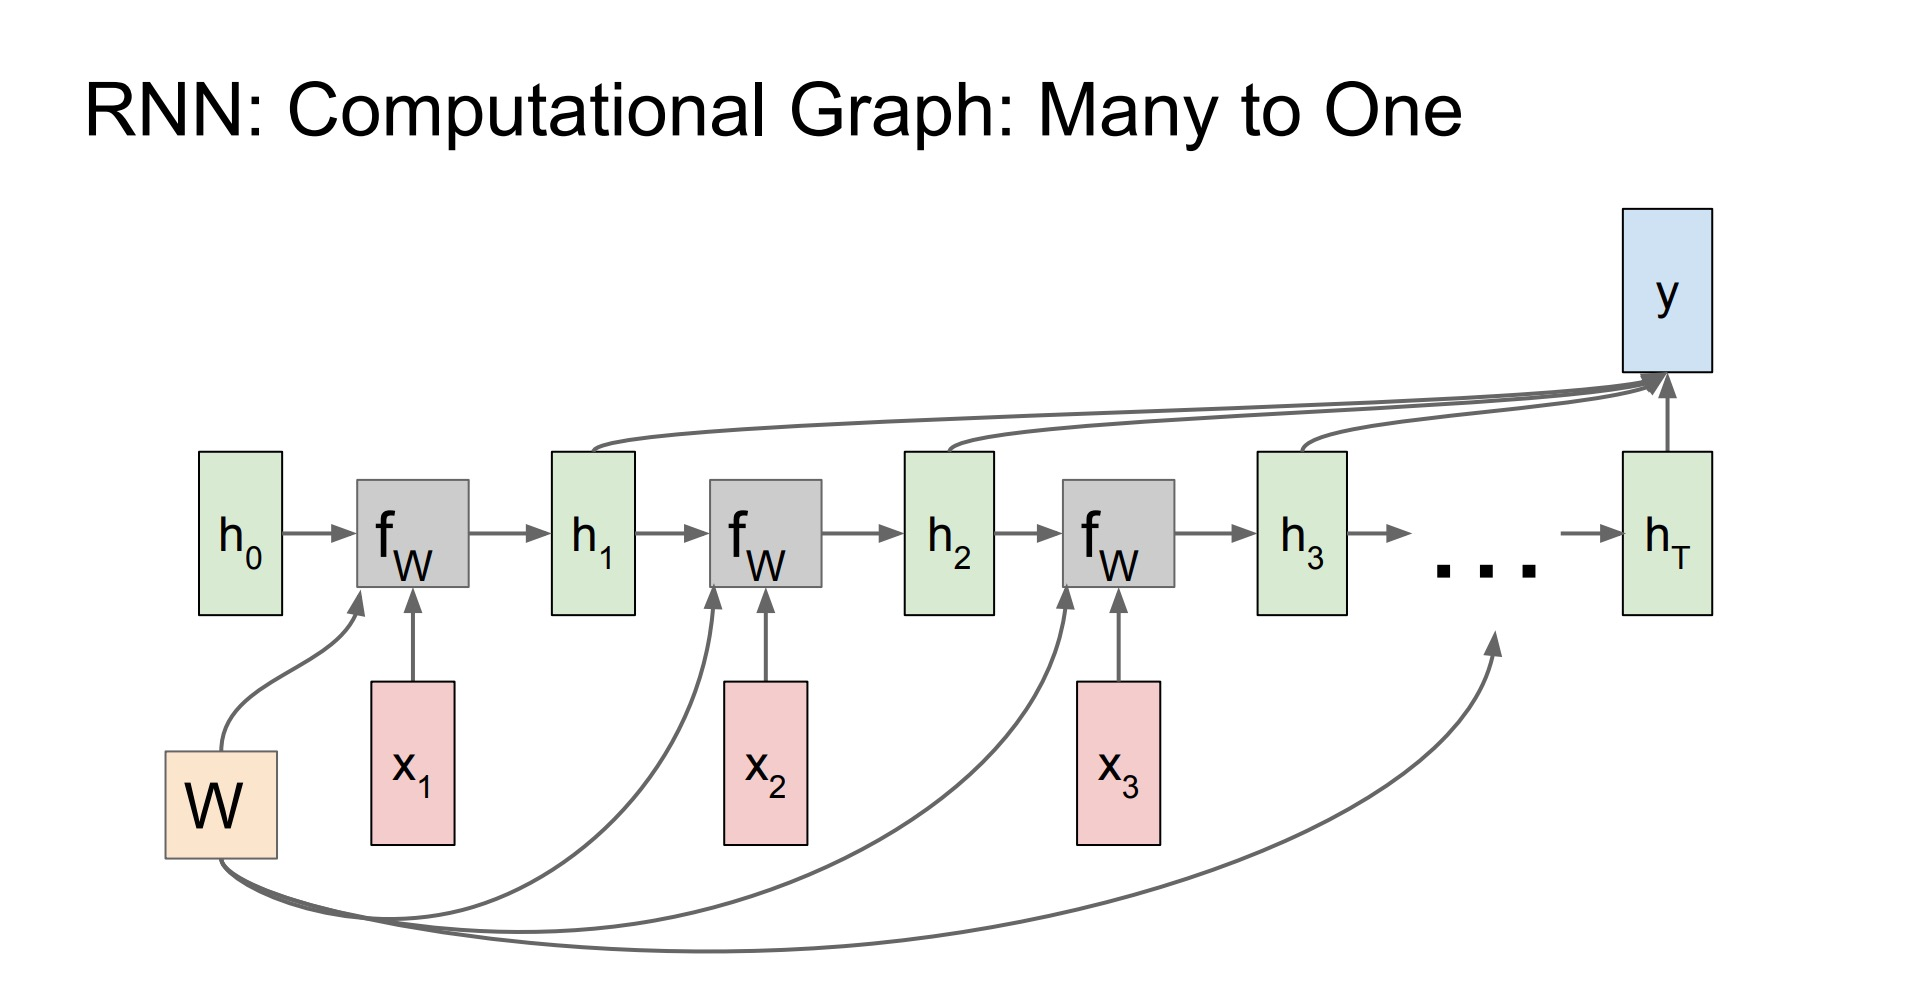
\includegraphics[width=0.45\linewidth]{figs/chapter5/cg mto.jpg} & 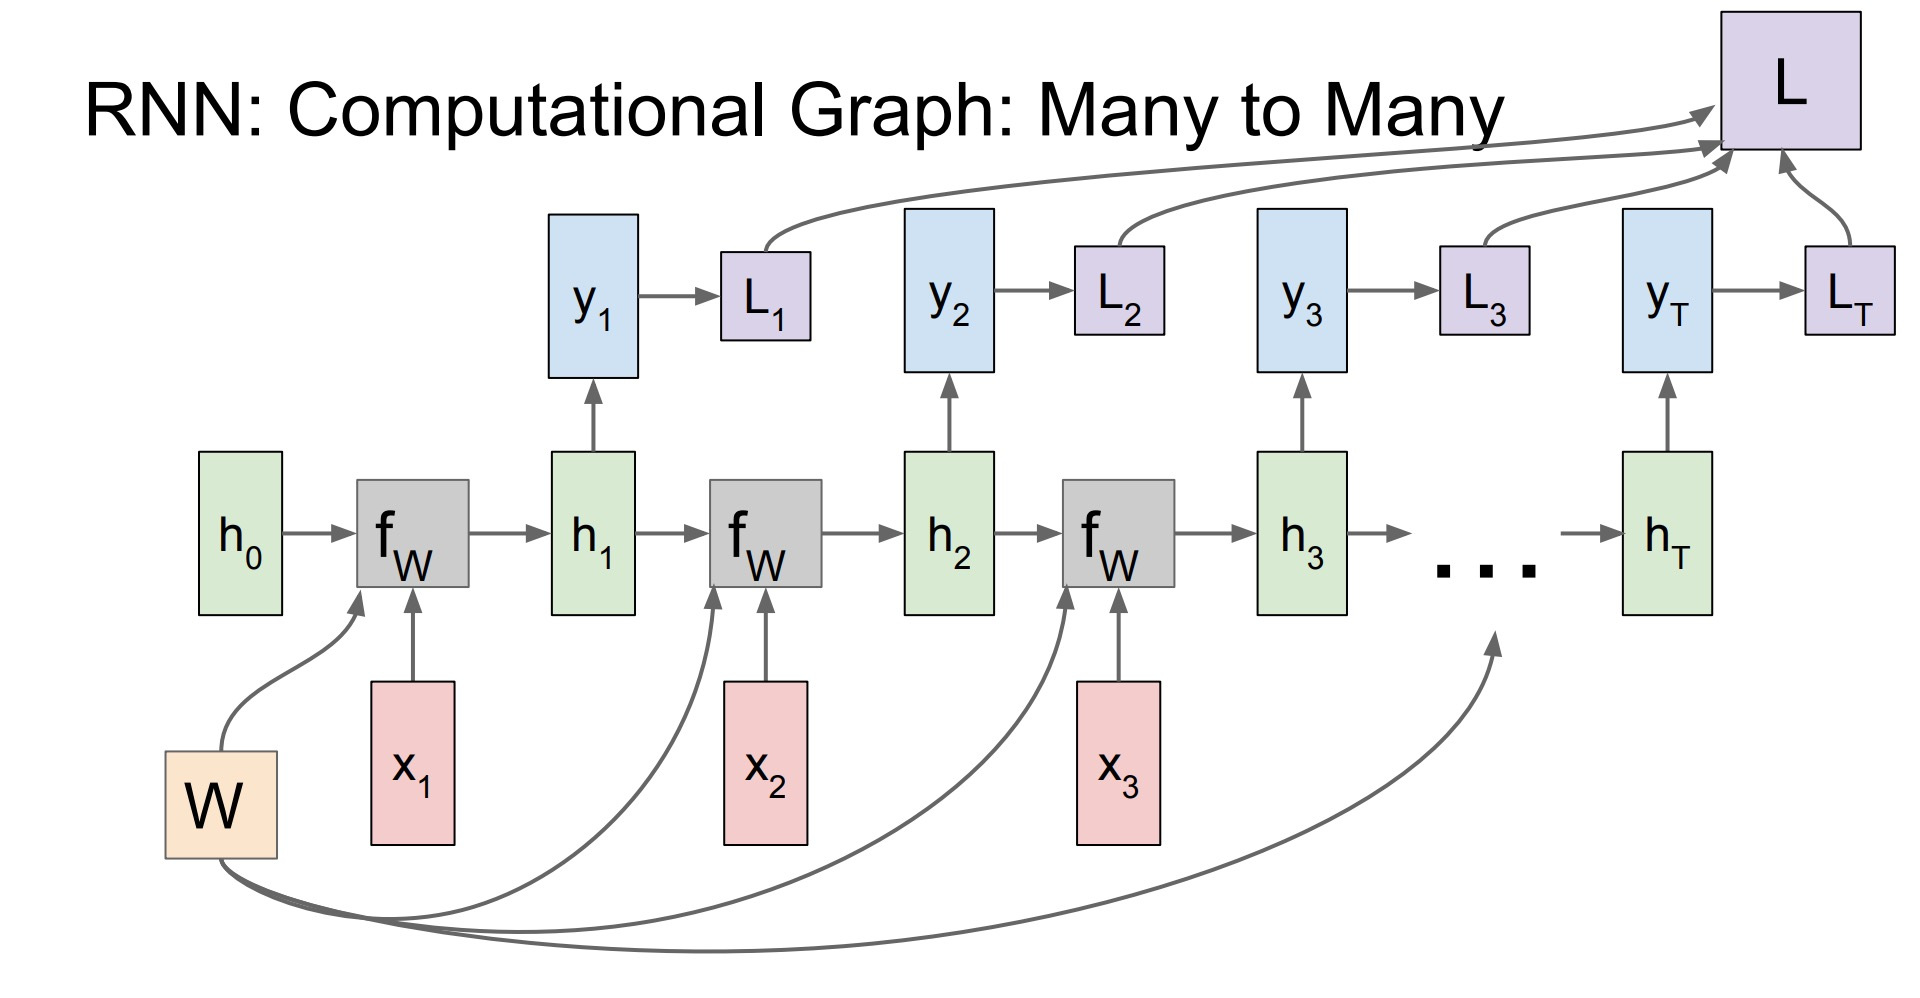
\includegraphics[width=0.45\linewidth]{figs/chapter5/cg mtm.jpg} \\
        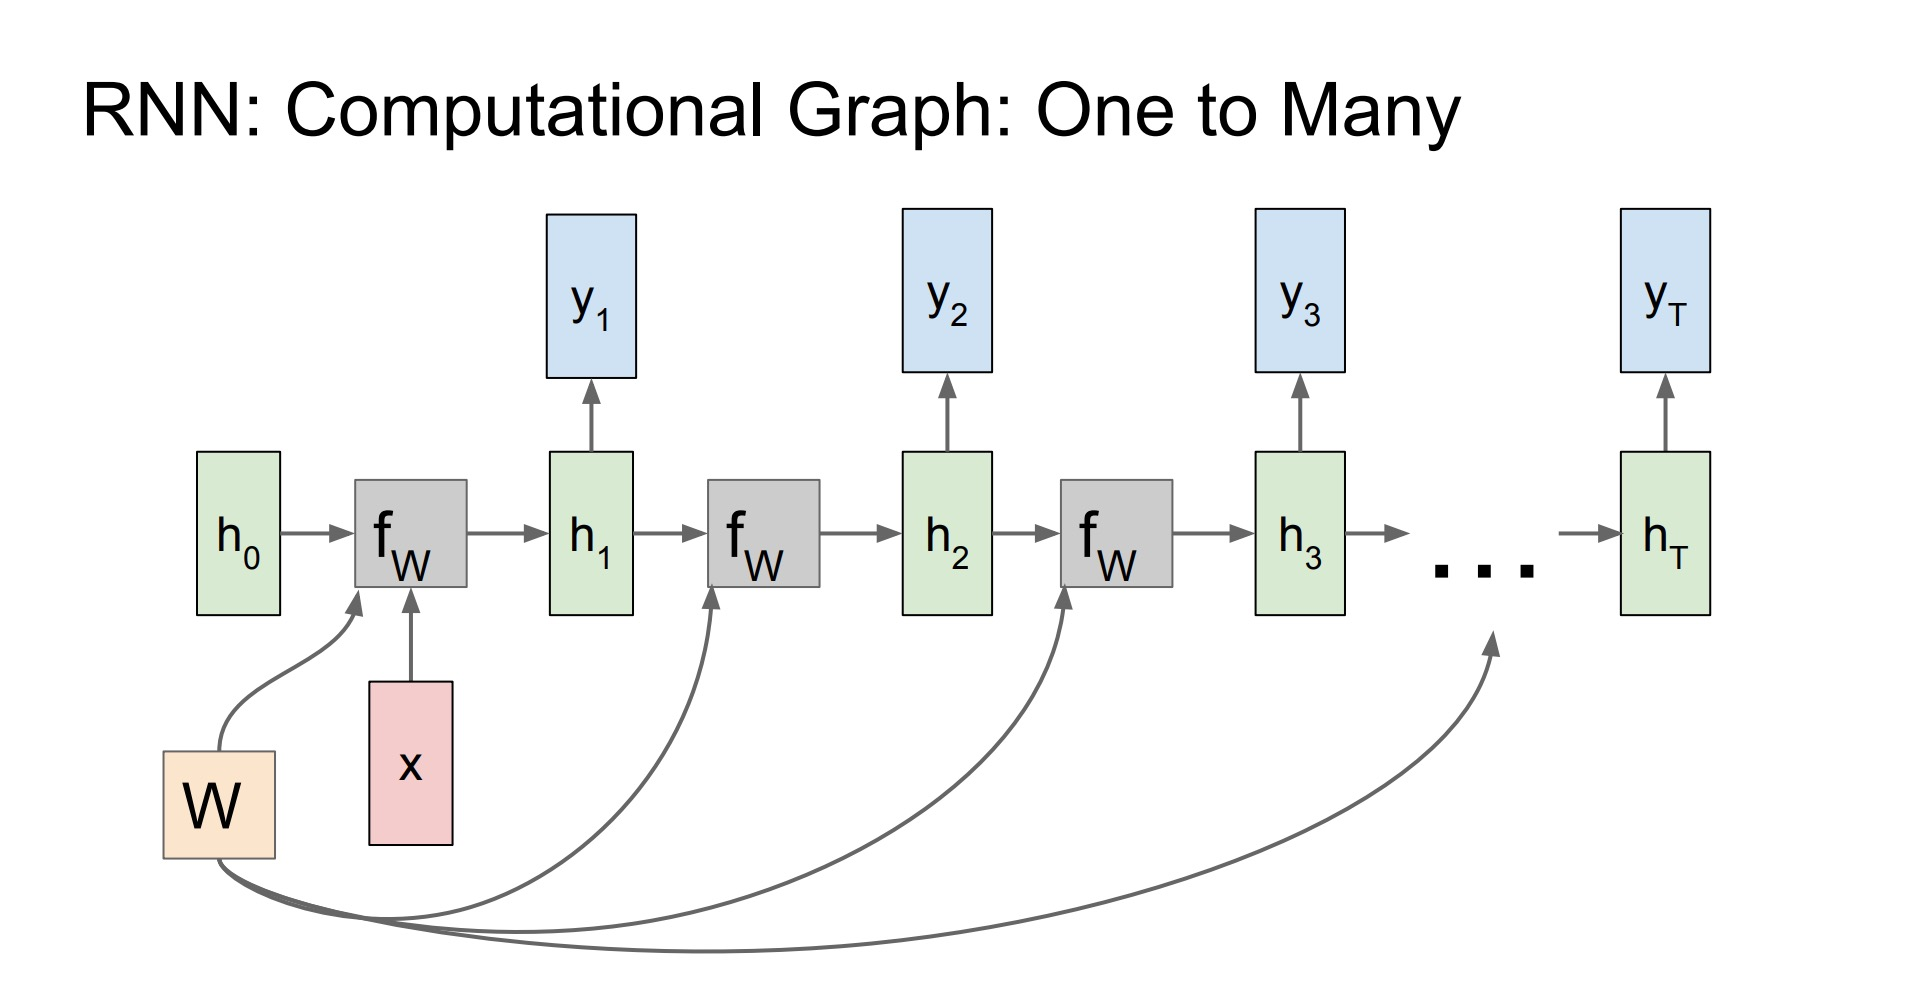
\includegraphics[width=0.45\linewidth]{figs/chapter5/cg otm.jpg} & 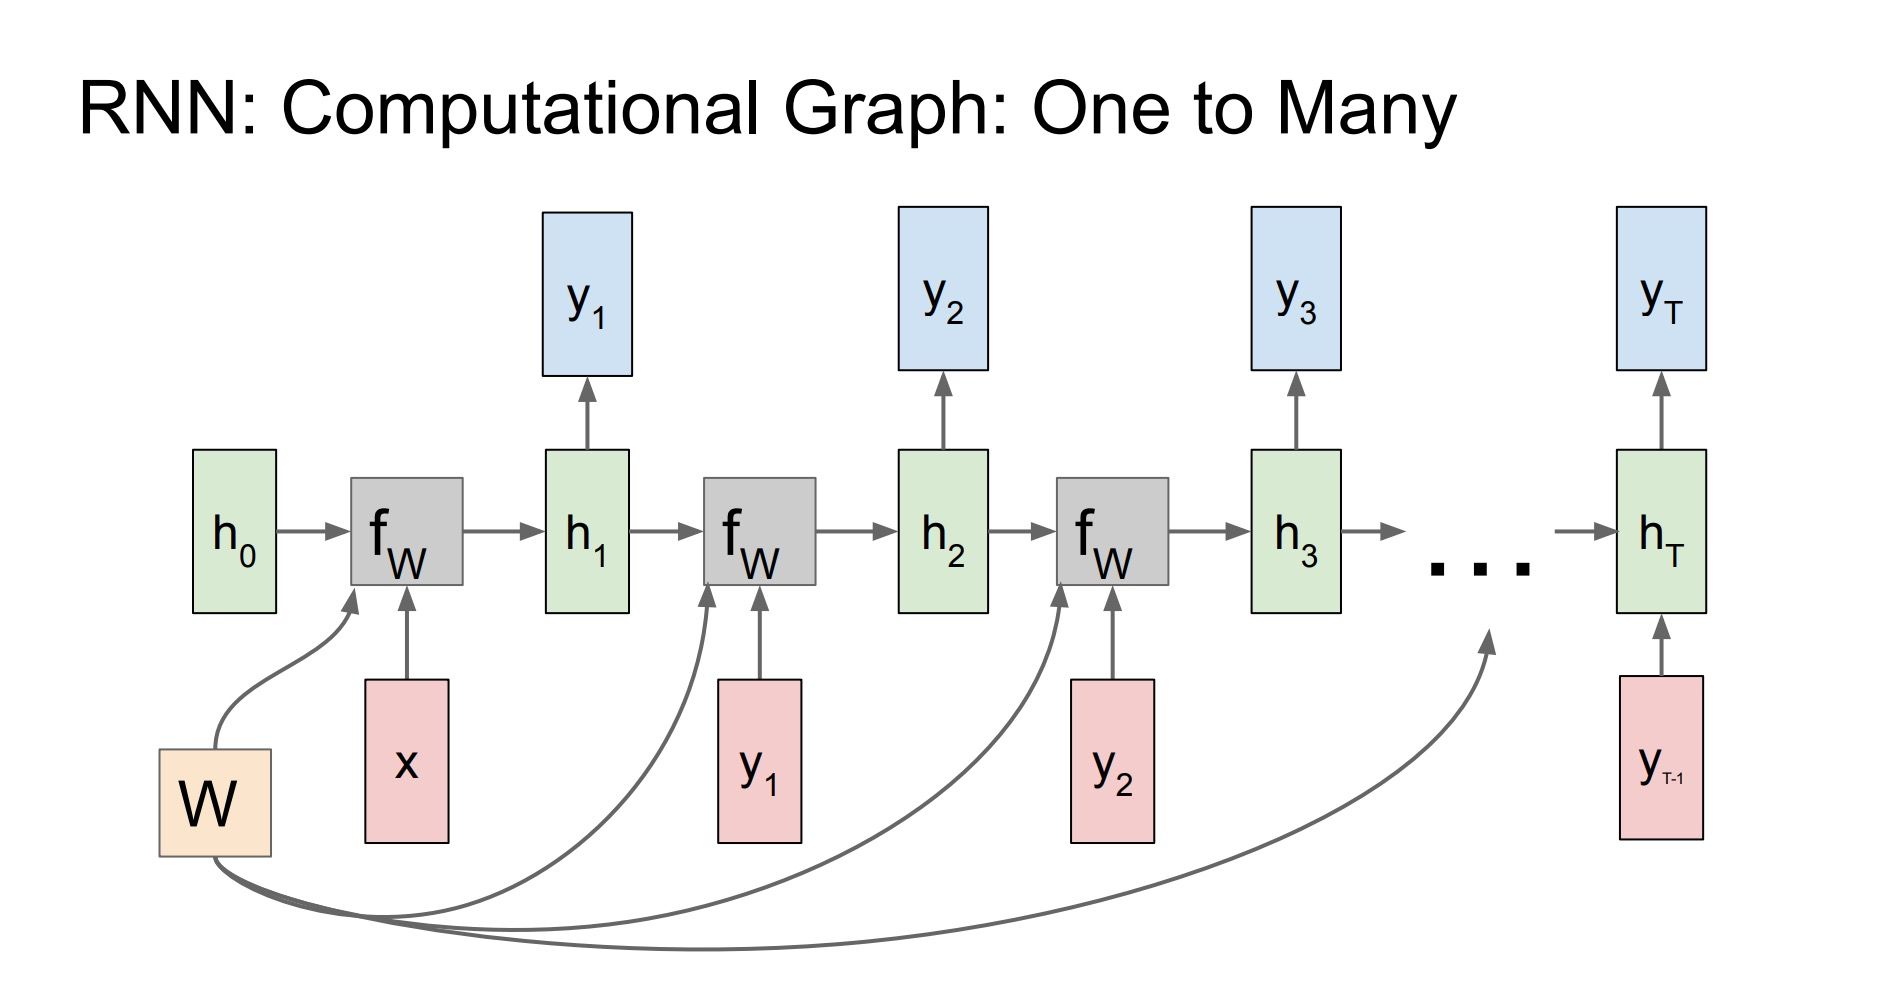
\includegraphics[width=0.45\linewidth]{figs/chapter5/cg otm2.jpg}
    \end{tabular}
\end{figure}

注意，在 one to many 结构中，我们可以用前一时刻的输出作为下一时刻的输入。

另外我们还可以把 many to one 和 one to many 连起来，形成 sequence to sequence 的效果。

\begin{figure}[H]
    \centering
    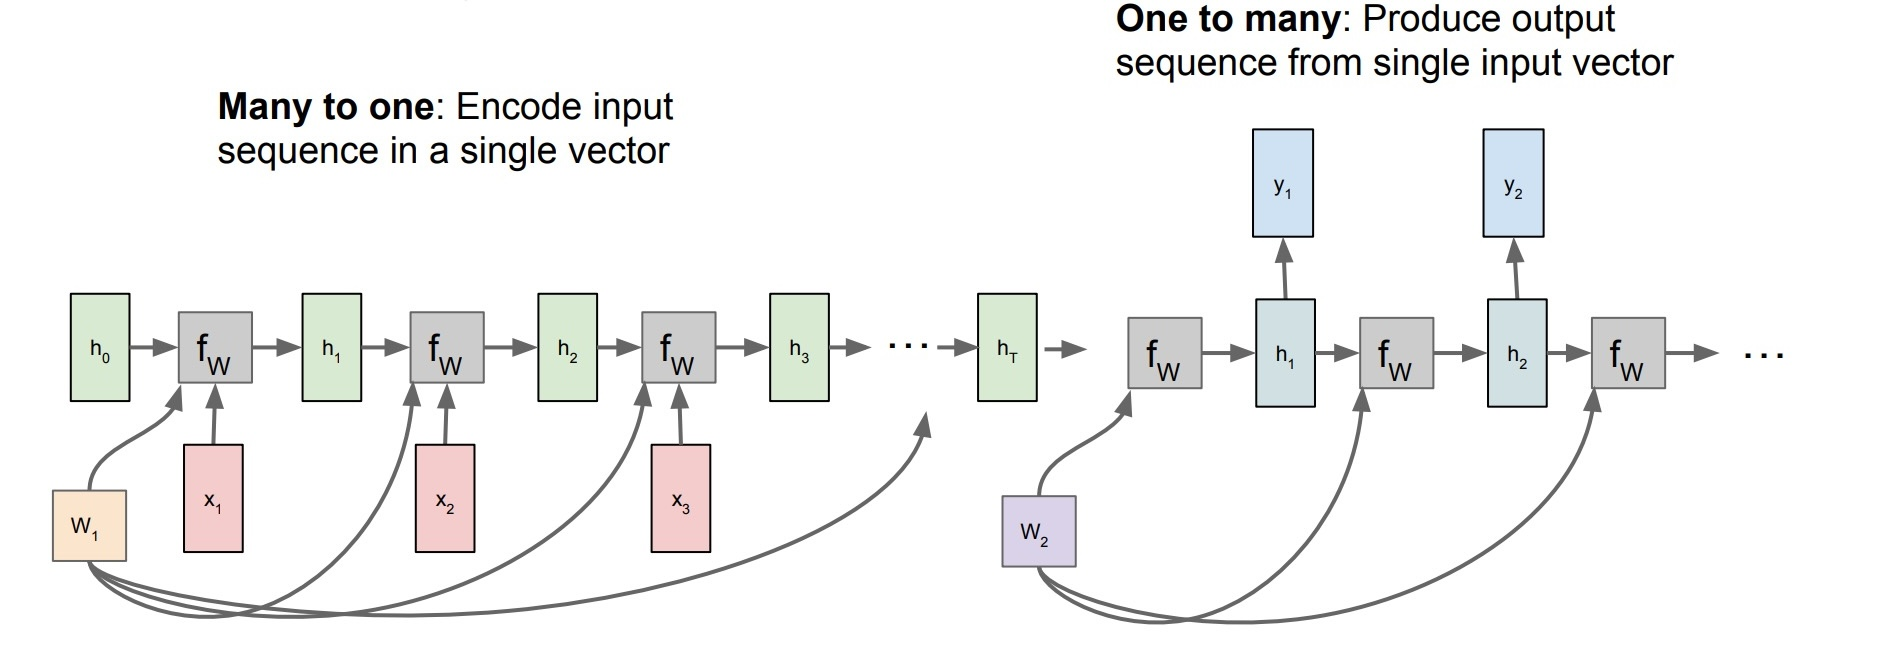
\includegraphics[width=0.8\linewidth]{figs/chapter5/cg sts.jpg}
\end{figure}

\paragraph{Backpropagation}
向前传播是按照时序计算的，于是反向传播就逆着时序传播。
\begin{figure}[H]
    \centering
    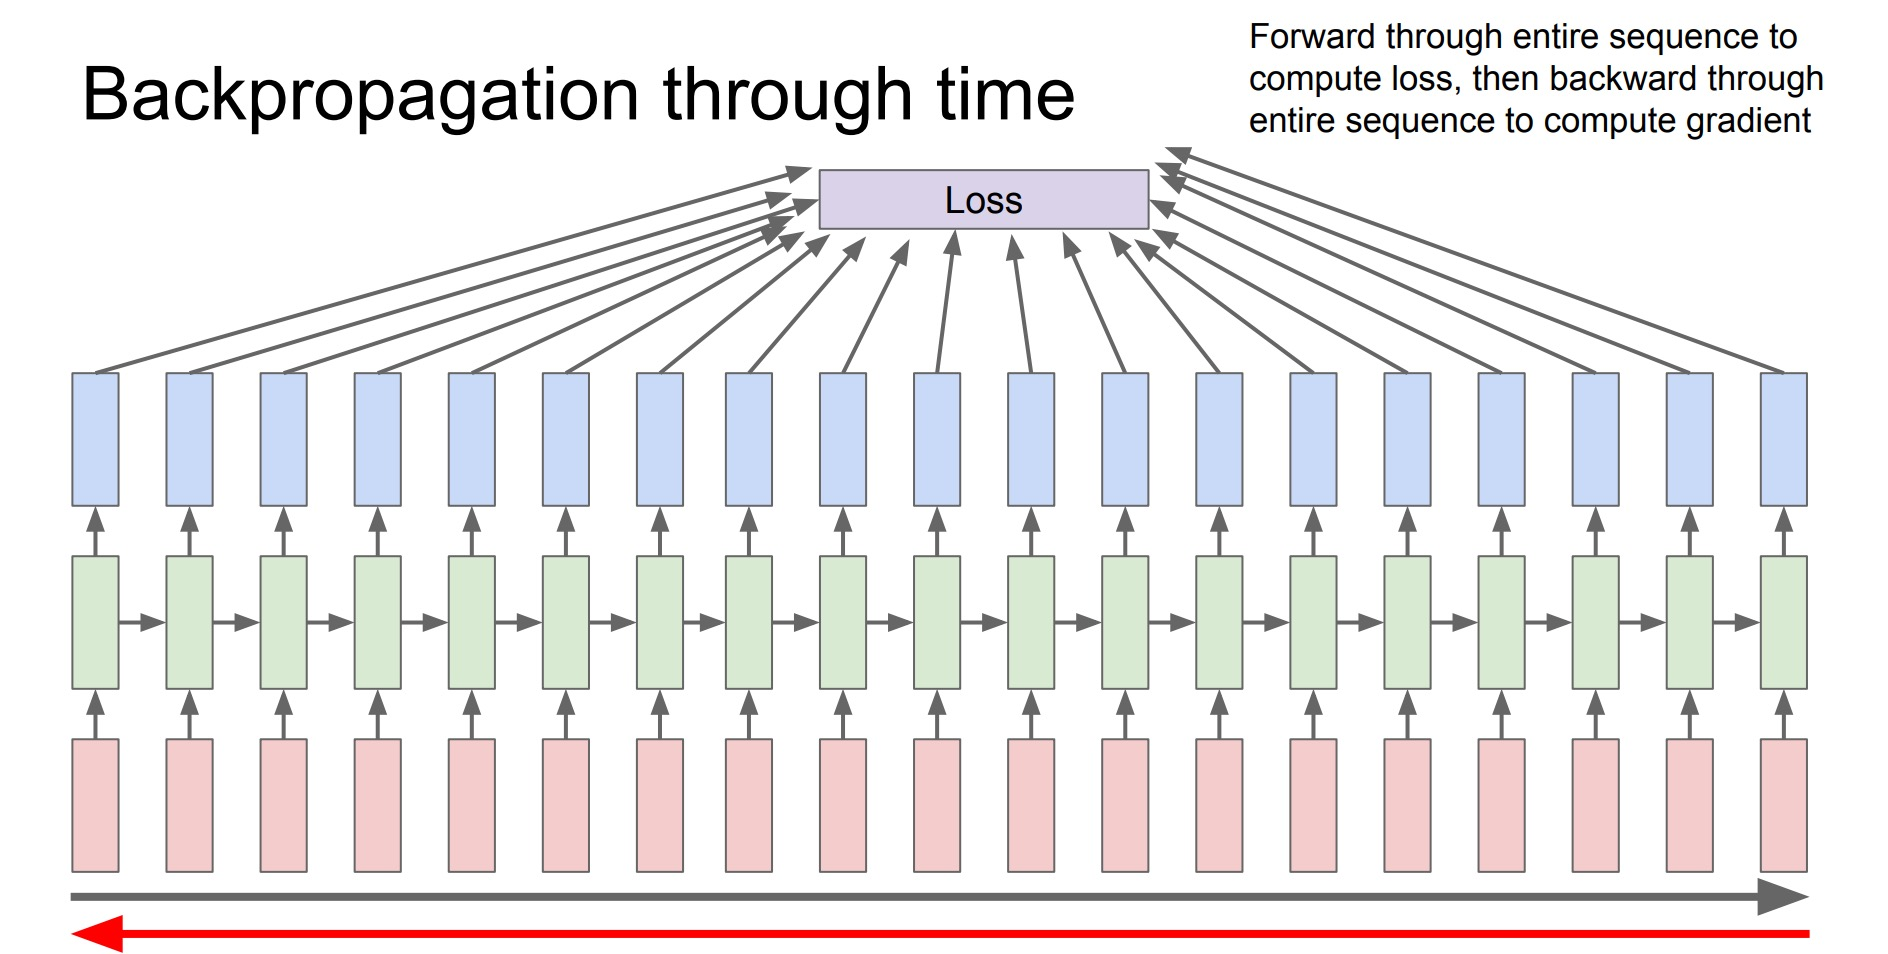
\includegraphics[width=0.7\linewidth]{figs/chapter5/bp.jpg}
\end{figure}
但是这里有一个问题，如果时序序列很长，这个过程会占用很大的内存。解决方案是 \textbf{Truncated} Backpropagation，把整个时序分段，每次向前传播一段后就对这段反向传播。
\begin{figure}[H]
    \centering
    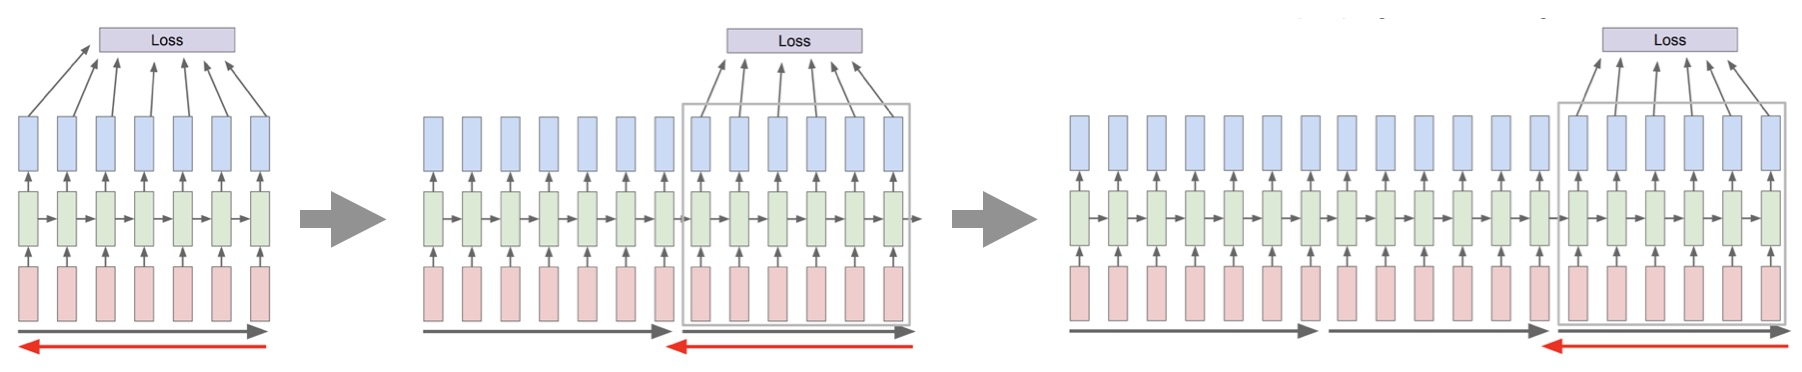
\includegraphics[width=1\linewidth]{figs/chapter5/Truncated.jpg}
\end{figure}

\paragraph{RNN Tradeoffs}

RNN 的优点有：

\begin{itemize}
    \item 可以处理任意长度输入。
    \item 时间步 $t$ 理论上可以使用前序时间步的所有信息。
    \item 模型大小不随输入长度的增加而增加。
    \item 每个时间步用同一套模型权重，对输入的处理存在一种对称性。
\end{itemize}

RNN 的缺点有：

\begin{itemize}
    \item 循环计算较慢
    \item 实际使用中，难以获取到非常多步之前的信息。
\end{itemize}

\subsection{LSTM (Long Short Term Memory)}

\paragraph{RNN Gradient Flow}

RNN 的在一个时钟中的更新为：
\[
h_t=\tanh(W_{hh}h_{t-1}+W_{xh}x_t)=\tanh\left(W\begin{pmatrix}h_{t-1}\\x_t\end{pmatrix}\right)
\]
\begin{figure}[H]
    \centering
    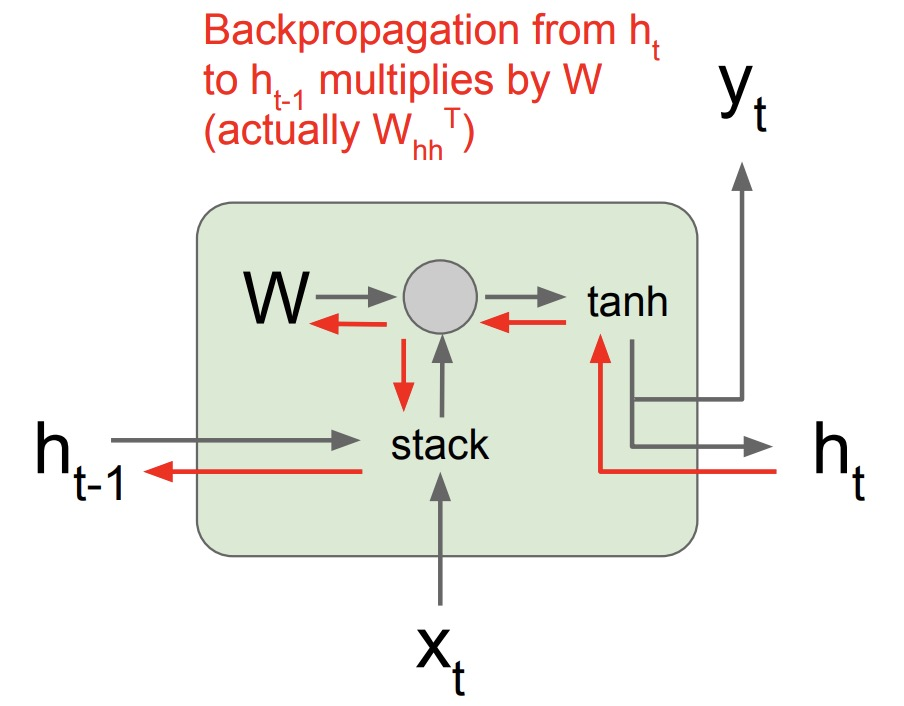
\includegraphics[width=0.3\linewidth]{figs/chapter5/rnngf1.jpg}
\end{figure}

在这一个时钟中，我们有：
\[
\frac{\partial h_t}{\partial h_{t-1}}=\tanh'\left(W_{hh}h_{t-1}+W_{xh}x_t\right)W_{hh}
\]
考虑整个时序：

\begin{figure}[H]
    \centering
    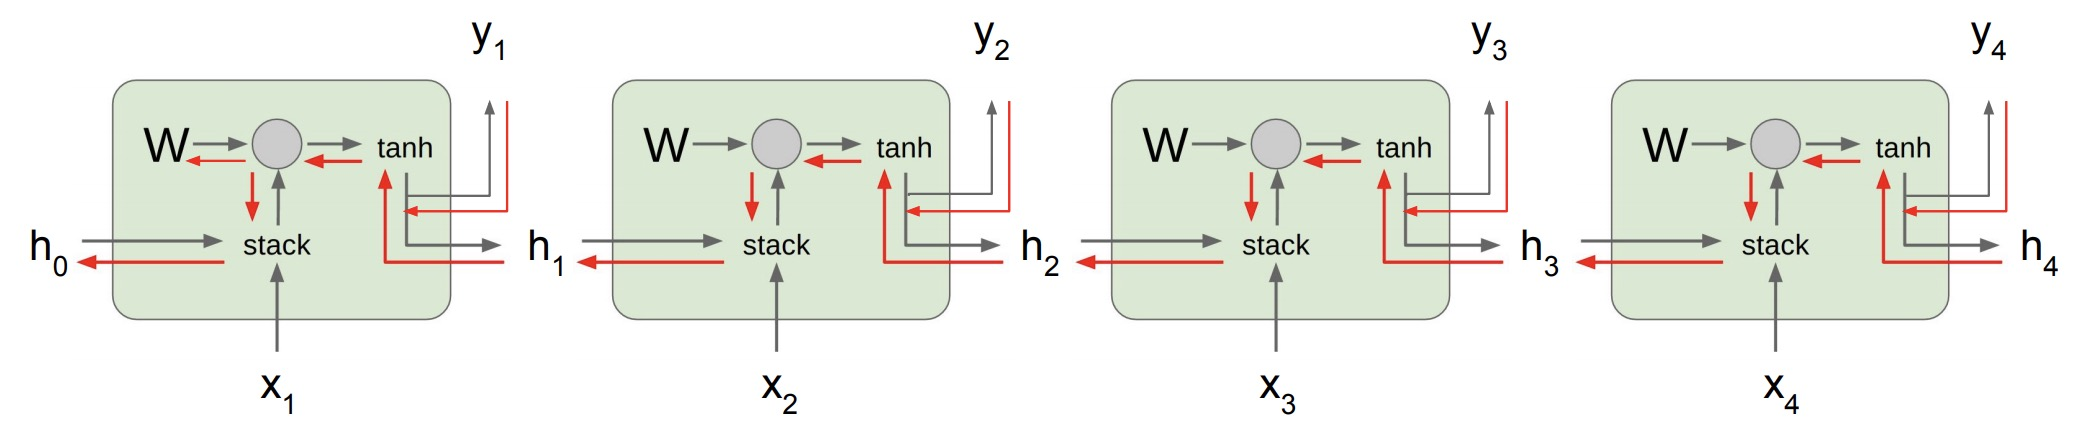
\includegraphics[width=1\linewidth]{figs/chapter5/rnngf2.jpg}
\end{figure}

我们 Backpropagation 的目的是找到 $\partial L/\partial W$：
\[
\frac{\partial L}{\partial W}=\sum_{t=1}^T\frac{\partial L_t}{\partial W}
\]
若仅考虑 $\partial L_T/\partial W$：
\begin{align*}
\frac{\partial L_T}{\partial W}&=\frac{\partial L_T}{\partial h_T}\frac{\partial h_T}{\partial h_{T-1}}\cdots\frac{\partial h_{2}}{\partial h_1}\frac{\partial h_1}{\partial W}\\
&=\frac{\partial L_T}{\partial h_T}\left(\prod_{t=2}^T\frac{\partial h_t}{\partial h_{t-1}}\right)\frac{\partial h_1}{\partial W}\\
&=\frac{\partial L_T}{\partial h_T}\left(\prod_{t=2}^T\tanh'(W_{hh}h_{t-1}+W_{xh}x_t)\right)W_{hh}^{T-1}\frac{\partial h_1}{\partial W}
\end{align*}
由于 $\tanh'(x)\leqslant 1$（当且仅当 $x=0$ 时取等），所以上式中括号内的乘积将非常小，这导致 \textbf{梯度消失}。
即便不考虑括号那一项，注意 $W_{hh}^{T-1}$ 这一项，如果 $W_{hh}$ 的最大奇异值 $>1$，该项将很大，导致 \textbf{梯度爆炸}；而如果 $W_{hh}$ 最大奇异值 $<1$，该项将很小，导致\textbf{梯度消失}。总而言之，梯度在 RNN 中的传播是困难的，于是我们思考改进 RNN 的结构来解决这个问题。

\paragraph{LSTM}

LSTM 在普通 RNN 的基础上多加了四个中间变量，将一个时钟中的更新定义为：
\[
\begin{cases}
&\begin{pmatrix}i\\f\\o\\g\end{pmatrix}=\begin{pmatrix}\sigma\\\sigma\\\sigma\\\tanh\end{pmatrix}W\begin{pmatrix}h_{t-1}\\x_t\end{pmatrix}\\
&c_t=f\odot c_{t-1}+i\odot g\\
&h_t=o\odot \tanh(c_t)
\end{cases}
\]
其中：

\begin{itemize}
    \item $i$: Input gate, whether to write to cell
    \item $f$: Forget gate, whether to erase cell
    \item $o$: Output gate, how much to reveal cell
    \item $g$: how much to write to cell

\end{itemize}
\begin{figure}[H]
    \centering
    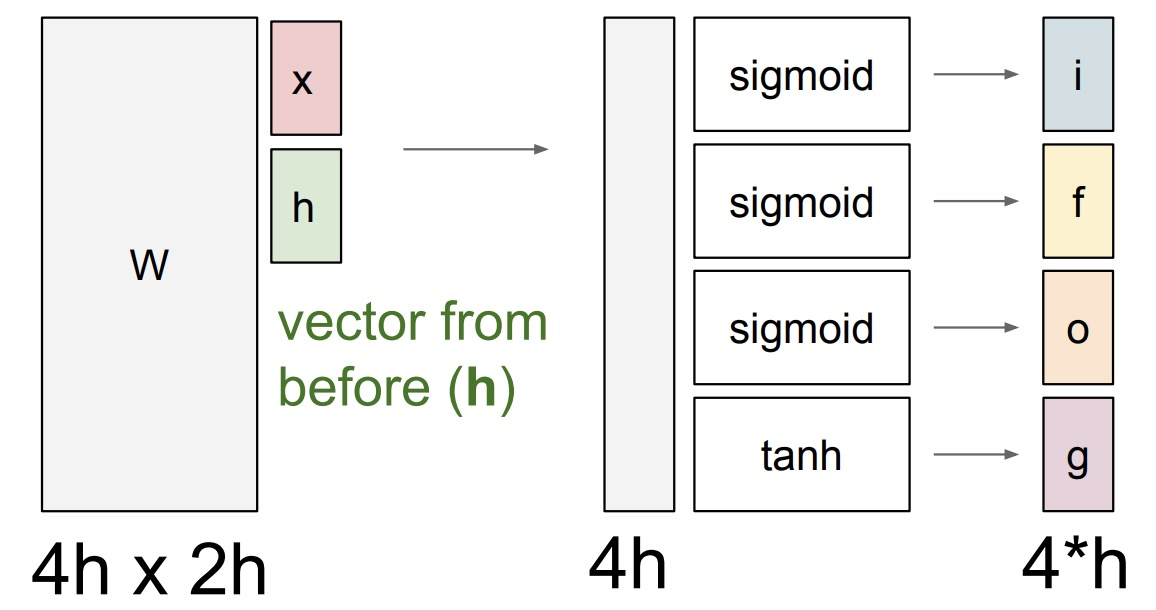
\includegraphics[width=0.4\linewidth]{figs/chapter5/lstm.jpg}
\end{figure}

注意，计算上述四个 gate 各自的 $W$ 是不同的，而上式中的 $W$ 表示把它们写在一起的矩阵。

在一个时钟中，LSTM 的从 $c_t$ 到 $c_{t-1}$ 的梯度更新为：

\begin{figure}[H]
    \centering
    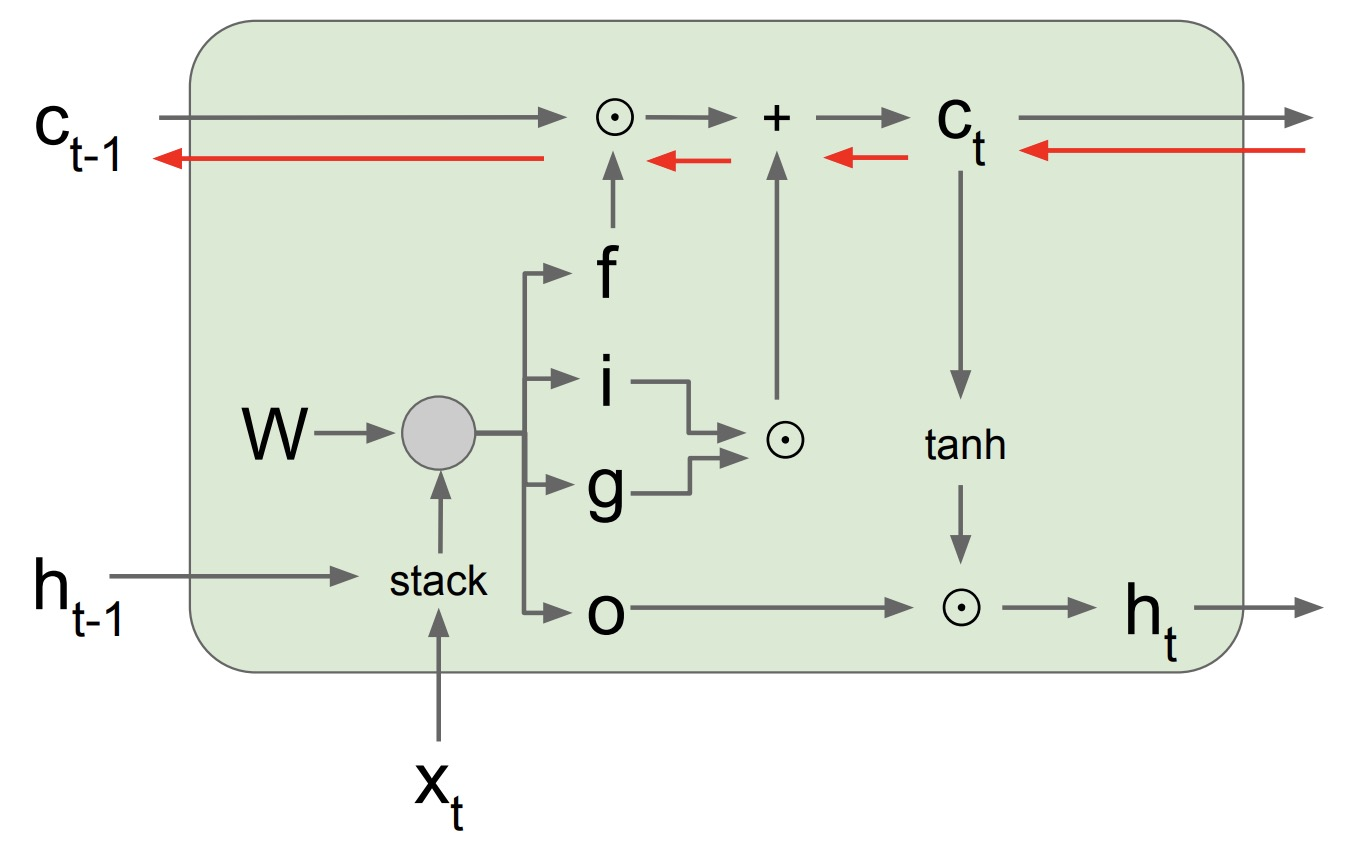
\includegraphics[width=0.3\linewidth]{figs/chapter5/lstmgf1.jpg}
\end{figure}

整个时序上，gradient flow 显得很顺畅：

\begin{figure}[H]
    \centering
    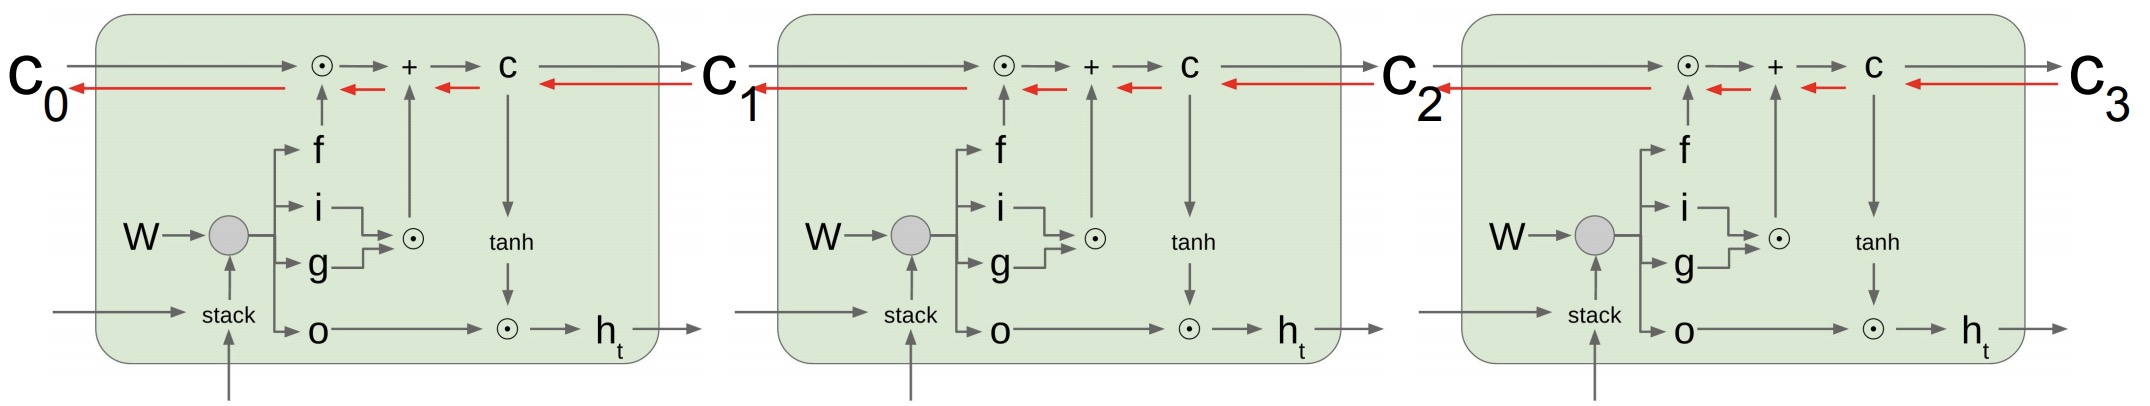
\includegraphics[width=0.9\linewidth]{figs/chapter5/lstmgf2.jpg}
\end{figure}

虽然 LSTM 不能保证不会发生梯度爆炸或梯度消失，但是它的 gradient flow 机制确实使得神经网络更容易训练。梯度在 LSTM 中的反向传播好似走了一条 high way，这一点上 LSTM 与 ResNet 有异曲同工之妙。
